\chapter{Experiential Learning of Networking Technologies: Understanding IP Routing}

\begin{center}
{\large\uppercase{$\text{Ram P. Rustagi}$}} 


\vskip -6pt

\end{center}

\vskip 2cm




\vfill




\newpage

\begin{multicols}{2}

In the previous article \cite{art2-key01}, we have studied assignment of IP address \cite{art2-key02} to a host, and its role in connecting to internet and communicating with other devices. We explored concept of a network number which is determined using IP address and subnet mask. When network number of two hosts is same, then these two hosts belongs to same network else these hosts belong to different networks. Hosts within the same network communicate directly with each other whereas hosts belonging to different network communicate using one or more intermediate routers. A router connects two networks, and its main job is to receive packets from one network and forward it to another network so as to enable the packet delivery towards its final destination. When two hosts are connected by many intermediate networks, communication between these two hosts require that each of the intermediate router in the path forward the packet on to the network which is closer to the destination and router in the last leg of this path will deliver the packet to destination host. In this article, we will explore this concept of packet forwarding and the mechanisms used to achieve this packet forwarding.

Consider the connectivity of two networks, say Network-1 and Network-2, as shown in Figure~\ref{chap2-fig01}. Each of these two networks consists of many connected systems (though as a representation only 2 are shown). Host $\textrm{H}_1$ and $\textrm{H}_2$ are part of Network-1, and Host $\textrm{H}_3$ and $\textrm{H}_4$ are part of Network-2. These two networks are connected via many intermediate routers, which we can consider as representing the internet. Host H1 and $\textrm{H}_2$ belongs to same network 10.x.x.0/24, and hence can communicate directly without requiring any intermediate router. Similarly, host $\textrm{H}_3$ communicates directly with $\textrm{H}_4$ as both belong to same network 10.y.y.0/24. However, when $\textrm{H}_1$ needs to communicate with $\textrm{H}_3$, the packets have to go through all the intermediate routers. When $\textrm{H}_1$ wants to send a packet to $\textrm{H}_3$, it will forward the packet to router $\textrm{R}_1$, which in turn will forward the packet to next router $\textrm{R}_2$, and so on, and finally Router $\textrm{R}_n$ will deliver the packet to host $\textrm{H}_3$. Thus, communication between two hosts involves routing of packets and primary focus of this article is to explore the mechanism used in forwarding these packets.

%~ \begin{figure}[H]
%~ \centering
%~ 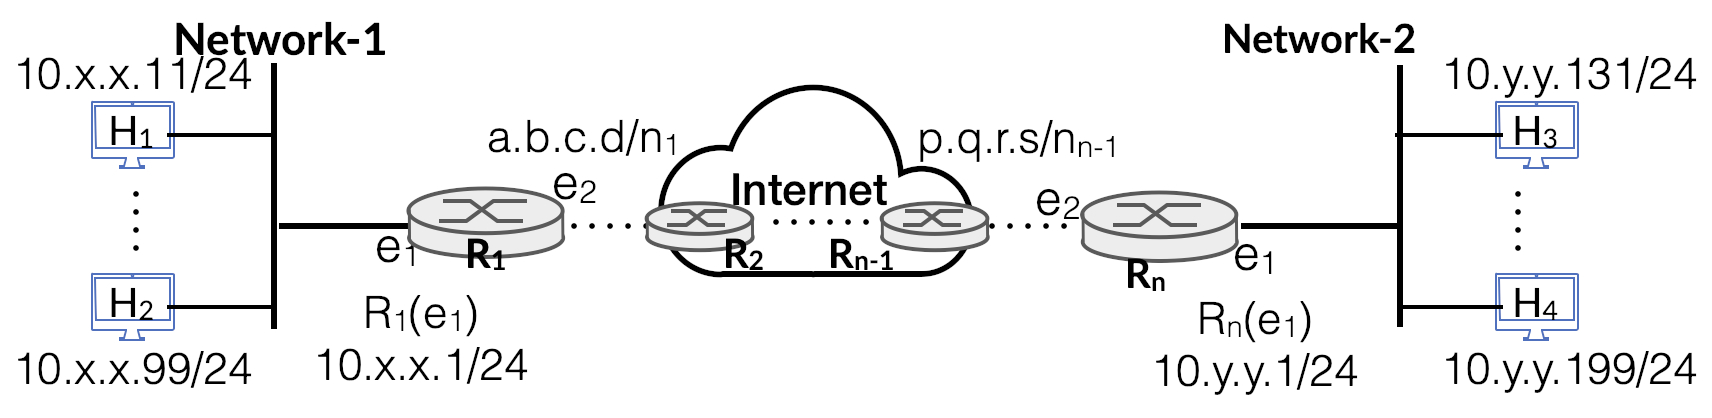
\includegraphics[scale=1.5]{src/Figures/chap2/chap2-fig01.jpg}
%~ \caption{Connectivity of two Networks, each network having many systems in it}\label{chap2-fig01}
%~ \end{figure}

Whenever, a host needs to send a packet to another hosts, it must know the IP address of destination host. For example, when we use browser to search at google.com, the machine where browser is running, finds the IP Address of gogole.com and then sets up TCP connection using IP address of google.com. When sending a packet, a host consults its routing table (also called as forwarding table) and determine the next hop in the path to destination host. Entries in the routing table plays a crucial role in how a host makes a packet forwarding decision. The routing decision using the routing table is always required irrespective of whether the destination host is in the same network or a different network.

\section{Routing Table Structure}\label{chap2-sec-1}

The main purpose of routing table is to help a host in determining the next hop where packet should be forwarded. The next hop could even be the next intermediate router or the final destination host itself. At its core, routing table has following four column fields, though in many implementations it may have some more information fields, such as cost metric etc., which we will not consider for our discussion.
\begin{itemize}
\item[i.] Destination Network.
\item[ii.] Subnet mask (for destination network).
\item[iii.] Network interface.
\item[iv.] Next hop or gateway router’s IP address.
\end{itemize}

A routing table would have number of row entries, with each row corresponding to a destination network. First two fields together identify a network, and are used to check if destination IP address of packet belongs to this network. If this entry matches, then packet is forwarded on the associated interface ($3^{rd}$ field) to the next hop ($4^{th}$ field). Next hop entry field is applicable when destination host is not connected to local network and identifies the IP address of next router in the forward path.  A typical set of entries for router $\rm{R}_1$ in Figure.~\ref{chap2-fig01} is given below in Table~\ref{chap2-table-1}, and routing entries for Host $\rm{H}_1$ is given in Table~\ref{chap2-table-2}.

\begin{table}[H]
\caption{Routing entries for $\rm{R}_{1}$}\label{chap2-table-1}
\begin{tabular}{|c|c|c|c|c|}
\hline
\textbf{S.N} & \textbf{Destination Network} & \textbf{Netmask} & \textbf{Interface} & \textbf{Next Hop}\\
\hline
1 & 10.x.x.0 &/24 & $\rm{e}_{1}$ & -\\
\hline
2 & a.b.c.d &/$\rm{n}_{1}$ & $\rm{e}_{2}$ & -\\
\hline
3 & \dots & \dots & \dots & \dots\\
\hline
4 & p.q.r.s & /$\rm{n}_{\rm{n}-1}$ & $\rm{e}_{2}$ & IP address of $\rm{R}_{2}$\\
\hline
5 & 10.y.y.0 & /24 & $\rm{e}_{2}$ & IP address of $\rm{R}_{2}$\\
\hline
6 & 0.0.0.0 & /0 & $\rm{e}_{2}$ & IP address of $\rm{R}_{2}$\\
\hline
\end{tabular}
\end{table}

\begin{table}[H]
\caption{Table 2: Routing entries for Host $\rm{H}_{1}$}\label{chap2-table-2}
\begin{tabular}{|c|c|c|c|c|}
\hline
\textbf{S.N.} & \textbf{Destination Network} & \textbf{Netmask} & \textbf{Interface} & \textbf{Next Hop}\\
\hline
1 & 10.x.x.0 & /24 & Ethernet & -\\
\hline
2 & 0.0.0.0 & /0 & Ethernet & 10.x.x.1\\
\hline
\end{tabular}
\end{table}

First two entries in Table~\ref{chap2-table-1} corresponds to two networks to which router $\rm{R}_{1}$ is directly connected and hence there is no next hop address. These will be followed by number of entries corresponding to network numbers that exist in the network. The entries in $4^{\rm th}$ and $5^{\rm th}$ row correspond to two networks connected with the router $\rm{R}_{n}$. Lastly, there is an entry corresponding to 0.0.0.0/0 which is also referred to as default route entry. Use of this default entry is explained ahead. For any host which is typically connected to a single network, there are generally two entries, as shown in Table~\ref{chap2-table-2} for host $\rm {H}_{1}$. One entry corresponds to local network and other entry corresponds to default network i.e. 0.0.0.0/0. These entries are sorted in the decreasing order of number of bits in netmask. For example, entry for netmask /27 will come before entries of netmask /26 or /25 etc.

\section{Using Routing Table to Forward Packets}\label{chap2-sec2}

When a host needs to send a packet to destination host or an intermediate router need to forward a received packet, then both the host and the router use a routing algorithm to determine how to send the packet to next hop or directly reachable destination host. An outline of such a routing algorithm is given in Table~\ref{chap2-table-3}. 

\begin{table}[H]
\caption{Routing Algorithm}\label{chap2-table-3}
\begin{tabular}{|cl|}
\hline
01: &  \#Algorithm For forwarding the packet\\
02: & Extract the destination address from the packet\\
03: & Repeat the following for each entry in routing table\\
04: & Apply the netmask ($2^{\rm nd}$ field) and compute network number\\
05: & Compare it with destination network ($1^{\rm st}$ field)\\
06: & If matche\\
07: & Forward packet to next-hop on listed interface ($3^{\rm rd}$ field)\\
08: & Exit // routing is over\\
09: & Else\\
10: & Continue to next entry\\
11: & When no match found (entry 0.0.0.0/0 not defined)\\
12: & Drop the packet\\
13: & Inform the sender (ICMP error message)\\
\hline
\end{tabular}
\end{table}

Consider the network given in Figure~\ref{chap2-fig01}, and that host ${\rm H}_{1}$ (belonging to Network-1) needs to send a packet to host ${\rm H}_{3}$ (belonging to Network-3). Thus the source and destination addresses of this packet would correspond to 10.x.x.11 and 10.y.y.131. Routing algorithm makes uses of only the destination address and does not consider the source address, and works as follows. Routing table of host ${\rm H}_{1}$ (Table~\ref{chap2-table-2}) has just two entries. Using the destination address 10.y.y.131 (as extracted from the IP packet in line 02 of), the lines 03 to 10 of routing algorithm will be applied to this destination address. Applying the netmask /24 of first entry in the routing table (Table~\ref{chap2-table-2}) to destination address 10.y.y.131 (line 04), network number is computed as 10.y.y.0. For a detailed discussion on computation of network number, reader can review the article by as given in \cite{art2-key01}. Comparison (line 05) of computed network number with destination network 10.x.x.0 for first entry fails and hence routing process repeats as per line 09-10 for the next entry. For the $2^{\rm nd}$ entry (Table~\ref{chap2-table-2}), netmask is /0, and applying this netmask to 10.y.y.131 gives the network number as 0.0.0.0. This computed network number matches with destination network in $2^{\rm nd}$ entry of routing table of ${\rm H}_{1}$, and thus packet is forwarded to router ${\rm R}_{1}$ on Ethernet interface of host ${\rm H}_{1}$. Applying netmask /0 with any IP address will always compute the network number as 0.0.0.0 and thus it will always match the destination network and therefore this is called the default route entry i.e. when no other routing entry matches, this entry will always match. The default route entry in a routing table always appears as the last entry.

\section{Delivering Packet to Next Hop and ARP Protocol}\label{chap2-sec3}

When host ${\rm H}_{1}$ is sending the packet to host ${\rm H}_{3}$, it only contains source IP address (${\rm H}_{1}$) and destination IP address (${\rm H}_{3}$). The packet does not have IP Address of either router ${\rm R}_{1-}$ or any of the intermediate router(s). So, it is important to understand the mechanism used in delivering this packet to router ${\rm R}_{1}$ (next hop address). Any system is connected to a network via its link layer adaptor e.g. ethernet interface. Each link layer adaptor has its link layer address, also known as MAC (Medium Access Control) Address for ethernet adaptors. MAC address is a popular term and thus in general, any link layer address is called as MAC address. The MAC address consists of 6 bytes and generally written in hexadecimal notation. Windows system use dash as separator of two bytes, and therefore, MAC address in a windows system will be shown as xx-xx-xx-xx-xx-xx. In Linux, colon(:) is used as the separator and thus MAC address is shown as xx:xx:xx:xx:xx:xx.  An interesting property of MAC address is that it is unique across the world i.e. no two adaptors can have same MAC Address. The MAC address is assigned by link adaptor manufacturer and entire MAC Address space is managed by IEEE (Institute of Electrical and Electronic Engineers). Thus, whenever anyone wants to manufacture the link layer adaptors, they need to get a block of addresses (corresponding to first 3 bytes of MAC address) from IEEE and assign the remaining 3 bytes uniquely to each of the adaptor that company will manufacture. Thus, MAC address is not configurable by a user and is fixed with the adaptor whereas IP address is user configurable and assigned by a network administrator.

Whenever a machine sends a packet, the packet goes out from the link layer adaptor, which inserts its MAC address as the source MAC address in the transmitted frame. The sender also needs to correctly fill the destination MAC Address field in the transmitted frame, which is required for receiving host to receive and process it.  When link layer adaptor of receiving host receives a frame, it compares the received destination MAC address in the frame with its own MAC Address. Only when two addresses match, the adaptor receives the frame, extracts the network layer packet and passes it on to host for further processing by upper layer network stack. If the MAC address match fails, then adaptor simply discards the frame and network layer will not even see this packet. A link layer adaptor also receives and processes all those frames which have destination MAC address set as broadcast MAC address (all bits in the MAC address field are set to 1) and written as FF:FF:FF:FF:FF:FF.

Thus, for host ${\rm H}_{1}$ to forward the packet to router ${\rm R}_{1}$ (Figure~\ref{chap2-fig01}), it must fill the MAC address of the network interface ${\rm e}_{1}$ of router in the transmitted frame. From the routing table, it only knows the IP address of router ${\rm R}_{1}$. The MAC address of ${\rm R}_{1}$(${\rm e}_{1}$) interface, let say it is ${\rm MAC}_{\rm R1(e1)}$, is known only to ${\rm R}_{1}$. Unless the sender host fills this MAC address in the frame being sent, ${\rm R}_{1}$ will never receive this packet. Thus, we
\end{multicols}
